\chapter{Theory}
This report assumes that the reader is familiar with the basics of machine learning.
This includes basic linear algebra, data preprocessing and model selection.
Further a basic understanding of how neural networks function is assumed,
including the basic concept of gradiant descent used for model training.

\section{Saliency maps}\label{sec:saliency_maps}
When training deep neural networks on image data,
it is often difficult to know exactly what the model is doing.
Especially in fields like medical image analysis,
where the classification of a model might influence if a patient is correctly diagnoed or not,
it is very desireable to know what the model is doing to be able to critique the model.

In image analysis, a tool to try to understand models are the so-called \textit{saliency maps}.
A saliency map is supposed to be a visual representation what parts of the image are important to the model,
when it made a given prediction.

For instance, in a model supposed to classify if a picture of a bone is broken or not,
we want the model to look at the bone and not really anything else in the image.

Many methods exist to produce saliency maps, each with their own strengths and weaknesses.
One of the most popular ones is the gradient based method (explained below).
This method is popular because it is computationally efficient and the implementation comes almost for free if Backpropagation is implemented.

\subsection{Gradient based saliency maps} \label{sec:gradiant_saliency_maps}
As described in Section \ref{sec:partial_derivatives_of_scalar_over_vector},
if a function $f: \mathbb{R}^n \rightarrow \mathbb{R}$ is defined,
then the gradient of $f$ in a point $x\in\mathbb{R}$ is a vector from $\mathbb{R}^n$.
A special case of this, is where $f$ is an image classification model, that takes
an image (images can be vectorized, hence still a vector) and returns a vector of probabilities for
diferent classes.
Then the gradient in any probabilty of the output vector, will be of the same size as the input vector.
Since the input vector was an image, the gradient can also be interpreted as an image.
It is this property that is utilized when calculating gradient based saliency maps.

Often, these gradients are used as heatmaps over the image, to hightlight regions that
supposedly contributed a lot to the classification decision of the model.
For instance in the book Interpretable Machine Learning (chapter 10.2)\cite{interpretable-machine-learning}, the gradient based
saliency map method is described to
''assign each pixel a value that can be interpreted as the relevance of the pixel to the prediction or classification of that image''.

One should however be careful with that intepretation, as the gradient is just poiting to/away from the classification boundary.
Recent research is pointing toward problems with the usage of saliency maps as explained in the quote before\cite{false-hope}.
This report will not go deeper into exactly what information that can be extracted from a gradient based saliency map,
but just note to be carefull when using them.

\section{The ResNet architecture}
The ResNet architecture is a popular architecture for deep neural networks.
It was presented in 2015 and presented some promising results on the ImageNet dataset\cite{RESNET-paper}.
The main idea in the architecture is to let some of the output from the internal convolutional layers
be \textit{fed forward} to layers a few layers deeper in the network.
The network is shown in Figure \ref{fig:resnet-18-architecture},
and the arrows show where the feed forward is happening.

\begin{center}
    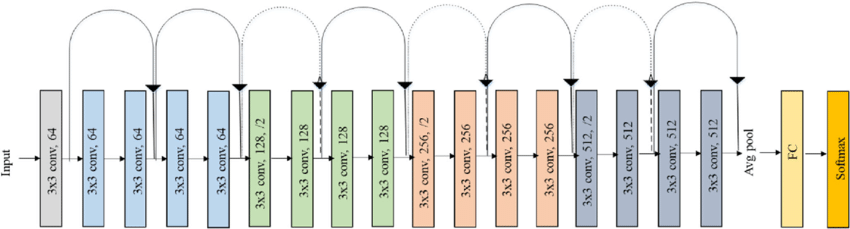
\includegraphics[width=0.9\textwidth]{images/ResNet-18-architecture.png}
    \captionof{figure}{ResNet-18 architecture. Figure taken from \cite{paper-with-resnet-18-figure}.
        The FC is short for Fully Connected layers, and the conv is short for convolutional layers. }
    \label{fig:resnet-18-architecture}
\end{center}


The architecture is implemented PyTorch\cite{PyTorch} and other similar libraries, making it easy to use.

\section{Model metrics} \label{sec:model_metrics}
To compare the performance of different models, different kinds of metrics can be used.
In the litterature on HAM10000, some researchers choose to look at all the classes presented
in Table \ref{table:ham10000}.
Others choose to only look at weather the lesion is benign or malignant
(see the \textit{severity} column in Table \ref{table:ham10000} - the \textit{pre-malignant} will be considered malignant).
To enable comparison with as many other studies as possible, we will report different metrics
on both problems as desribed in the following.
\subsection{Multiclass accuracy}
The most simple metric used here, is the accuracy, which is the percentage predictions that are correct.
\[
    \text{Accuracy} = \frac{\text{correct classifications}}{\text{total predictions}}
\]
Accuracy as a metric is not that good for problems with big class imbalance,
such as this one where a single class accounts for more than half of the data (see Table \ref{table:ham10000}).

\subsection{Binary accuracy}
The binary accuracy is defined exactly as the multiclass, but except of using all $7$ classes,
the considered classes are just benign and malignant.

\subsection{Malignant recall}
The general definition of recall in a binary classification problem is the percentage of the positive class
that is correctly classified.
The recall is defined as
\[
    \text{Recall} = \frac{\text{TP}}{\text{TP} + \text{FN}}
\]
Here $TP$ is the number of true positives, and $FN$ is the number of false negatives.
When refering to \textit{malignant recall}, we will think of the recall metric in the problem
where the considered classes are just benign and malignant.
As the name suggest, the positive class is malignant.

An intuitive way of thinking about this is how big a portion of the malignant lesions
that the model was able to detect.
On its own, a very high malignant recall does not mean the the model is very good,
as one can trivially make it $1$ by just having a model that always predicts malignant no matter the image.

\subsection{Malignant F1 score}
In general the F1 score is defined as
\[
    \text{F1 score} = \frac{2 \cdot \text{Precision} \cdot \text{Recall}}{\text{Precision} + \text{Recall}}
\]
giving rise to the need of for positive class, as the definition of recall requires one.
Here the \textit{Malignant F1 score} is defined as
\[
    \text{Malignant F1 score} = \frac{2\cdot \text{Precision} \cdot \text{Malignant recall}}{\text{Precision} + \text{Malignant recall}}
\]

A benifit of the F1 score is that it is a good metric to compare the performance of different models,
as it both takes the class imbalanance into account but also just the general performance of the model.

\subsection{Multiclass F1 score}
Defining a multiclass F1 score, is a bit more complicated than for a binary one.
The Python package that is used to calculate the F1 score in this project, \verb|sklearn|
\cite{sklearn}, has a mandatory parameter \verb|average|, that changes the way the F1 score is calculated.
In Figure \ref{fig:sklearn-f1-average-docs} the average parameter is described.
In this project, the we will use \verb|average='weighted'|, where the F1 score is calculated
using each of the classes in the problem as a positive class and then doing a weighted average of them based
on the number of samples in each class.
The reason for this choice, is that it explicitly considers the class imbalanance,
which is important for the multiclass problem on the HAM10000.


\begin{center}
    \begin{minted}{text}
    average : {'micro', 'macro', 'samples','weighted', 'binary'} or None, \
            default='binary'
        This parameter is required for multiclass/multilabel targets.
        If ``None``, the scores for each class are returned. Otherwise, this
        determines the type of averaging performed on the data:

        ``'binary'``:
            Only report results for the class specified by ``pos_label``.
            This is applicable only if targets (``y_{true,pred}``) are binary.
        ``'micro'``:
            Calculate metrics globally by counting the total true positives,
            false negatives and false positives.
        ``'macro'``:
            Calculate metrics for each label, and find their unweighted
            mean.  This does not take label imbalance into account.
        ``'weighted'``:
            Calculate metrics for each label, and find their average weighted
            by support (the number of true instances for each label). This
            alters 'macro' to account for label imbalance; it can result in an
            F-score that is not between precision and recall.
        ``'samples'``:
            Calculate metrics for each instance, and find their average (only
            meaningful for multilabel classification where this differs from
            :func:`accuracy_score`).
    \end{minted}
    \captionof{figure}[Cutout from sklearn documentation for F1 score]{
        Documentation for the required \textit{average} parameter for the F1 score in a multiclass problem
        (Copied from \url{https://scikit-learn.org/stable/modules/generated/sklearn.metrics.f1_score.html
        })}
    \label{fig:sklearn-f1-average-docs}
\end{center}


\section{Statistical tests with conditioned variables}\label{sec:statistical_tests_with_conditioned_variables}
% TODO: Write about statistical tests with conditioned variables
% http://users.stat.umn.edu/~helwig/notes/ChiSquareTests_slides.pdf
% there are good examples with white/black death penalty which seem to be 
% the standard example